\documentclass[letter,openright,12pt]{book}
\usepackage[spanish]{babel}
\usepackage[bookmarks]{hyperref}
\usepackage[utf8]{inputenc}
\usepackage{lmodern}
\usepackage{graphicx}
\usepackage{epstopdf}
\usepackage{array}
\graphicspath{ {./imagenes/} }
\setcounter{secnumdepth}{3} % para que ponga 1.1.1.1 en subsubsecciones...
\setcounter{tocdepth}{3} % para que añada las subsubsecciones en el indice...

\begin{document}

  \begin{titlepage}

    \begin{center}
      \vspace*{-1in}
      \begin{figure}[htb]
    \begin{center}
      
\includegraphics[width=8cm]{imagenes/Logo_Distrital.eps}
    \end{center}
    \end{figure}

    FACULTAD DE INGENIERÍA\\
    \vspace*{0.15in}
    PROYECTO CURRICULAR DE INGENIERÍA DE SISTEMAS \\
    \vspace*{0.6in}
    \begin{large}
    Tesis:\\
    \end{large}
    \vspace*{0.2in}
    \begin{Large}
    \textbf{EL TÍTULO DE LA TESIS} \\
    \end{Large}
    \vspace*{0.3in}
    \begin{large}
    Presentada por:\\
      Nicolás Mauricio Garcia Garzon 20091020031 \\
      Luis Felipe Gonzalez Moreno 20091020035
    \end{large}
    \vspace*{0.3in}
    \rule{80mm}{0.1mm}\\
    \vspace*{0.1in}
    \begin{large}
    Dirigida por: \\
    \end{large}
    \end{center}

    \end{titlepage}



  \newpage
  \mbox{}
  \thispagestyle{empty} % para que no se numere esta página
  
  
  \chapter*{Resumen} % si no queremos que añada la palabra "Capitulo"
  \addcontentsline{toc}{section}{Resumen} % si queremos que aparezca en el índice
  \markboth{RESUMEN}{RESUMEN} % encabezado
  
  \tableofcontents % indice de contenidos

  \cleardoublepage
  \addcontentsline{toc}{chapter}{Lista de figuras} % para que aparezca en el indice de contenidos
  \listoffigures % indice de figuras

  \cleardoublepage
  \addcontentsline{toc}{chapter}{Lista de tablas} % para que aparezca en el indice de contenidos
  \listoftables % indice de tablas
  
  \chapter{Definición del problema}
  
  \chapter{Justificación del problema}
  
  \chapter{Objetivos}
  \section{Objetivo General}
  \section{Objetivos especificos}
  
  \chapter{Hipotesis}
  
  \chapter{Marco teórico}
  
  \chapter{Metodología}
  
  \chapter{Metodos utilizados}
  
  A continuación se muestra el método utilizado para la recaudación de datos valiosos que soportara las decisiones de escogencia de deportes, publico objetivo y tecnología a aplicar.

\section{Encuesta inicial}

Con el fin de definir el grupo focal de la aplicación a desarrollar, se practicó una encuesta inicial por medio de internet. Gracias a esta encuesta, se pudo qué deportes son los mas populares, los menos populares, y de qué forma los jóvenes interactuan para practicar estos deportes. Teniendo en cuenta que el objetivo final de la aplicación es ayudar a que la práctica deportiva se masifique, se decidio que inicialmente no se van a tener en cuenta los deportes más populares (Futbol, Baloncesto, Ciclismo) e implementar la aplicación para que soporte los deportes menos populares. En este orden de ideas, los deportes seleccionados como pioneros en la aplicacion son el Rugby y el Tenis.

\subsection{Análisis de resultados}

La encuesta alcanzó un número de 155 personas. Ésta encuesta fue hecha por medio de internet, valiendose de grupos y sitios web que frecuentan los jóvenes de Bogotá, en su mayoría estudiantes universitarios (debido a nuestro alto interés en alcanzar personas sobre el rango de edad que presentan en \cite{user_behavior_online}).\\

\begin{itemize}
  \item Edad \\
  Los rangos de edad de los encuestados varían de 13 hasta 60 años, concentrándose en el rango de 20 a 27 años. Aún cuando esta pregunta no refleja ningún comportamiento de análisis, refleja que la encuesta fue practicada, en su gran mayoría, a los jóvenes Bogotanos.
  \item Ocupación \\
  Se puede apreciar como el 66\% de los encuestados son estudiantes. Los estudiantes suelen tener grupos de amigos/conocidos en su lugar de estudio con quienes pasan tiempo por fuera de sus lugares de estudio, son jóvenes que, en su mayoría, están disfrutando de su etapa de estudiantes universitarios, concentrándose mayoritariamente en sus estudios. Por otra parte, un 25\% de los encuestados dicen ser Empleados, y teniendo en cuenta como y a quien se le realiza la encuesta, se puede suponer que son estudiantes que, a parte de estudiar, también tienen que trabajar.
  \item Elementos electrónicos \\
  El elemento que mas  dicen tener los encuestados es el computador portátil (37\%) , lo cual tiene sentido teniendo en cuenta las necesidades de un estudiante universitario, seguido muy de cerca del computador de escritorio (26\%) y el smartphone (26\%). En la mayoría de los casos, aseguran tener tanto computador portátil como smarthpone. De allí se puede deducir que a los jóvenes les gusta estar en constante conexión con el mundo digital y la internet.
  \item Lugar de acceso a internet \\
  El lugar desde el que se accede a internet con mayor frecuencia es el hogar con un 43\%, seguido de el lugar de estudio (23\%) y del internet móvil(13\%). Adicionalmente, los encuestados aseguran que los lugares en los que duran mas tiempo conectados son el hogar (72\%) y el internet móvil (15\%). Esto muestra que hay preferencia en conectarse desde lugares y dispositivos en los que se sienten mas en privado (o en control) de quienes tienen acceso a la información contenida por estos dispositivos.
  \item ¿Practica deporte? \\
  El 63\% de los encuestados asegura practicar algún deporte, mientras el 37\% no. Las razones por las que este importante porcentaje de la población no practican algún deporte sale del alcance de esta primera encuesta.
  \item Deportes practicados \\
  En los deportes practicados, resaltan el Fútbol (27\%), Baloncesto (13\%) y Ciclismo (13\%), mientras que los deportes en los que se requieren implementos o lugares especializados no son tan comunes (Tenis 7\%, Escalada deportiva 3\%, Patinaje 1\% y no se practican deportes como Rugby, Fútbol Americano o Golf)
  \item Métodos de búsqueda \\
  Para analizar los métodos de búsqueda, se realizaron preguntas enfocadas a la búsqueda de nuevos deportes, implementos, lugares y grupos o equipos para practicar estos deportes. El común denominador para cada una de ellas fue consultar con los amigos, en donde siempre fue de las opciones mas populares, solo superada por la consulta de tiendas deportivas (en el caso de la búsqueda de implementos) y el CouchSurfing (en el caso de la búsqueda de un nuevo deporte), demostrando que las opiniones de los amigos/conocidos tienen mayor importancia que cualquier otra forma de búsqueda.
\end{itemize}



  
  \chapter{Cronograma}
  
  \chapter{Recursos}
  
  \section{Recursos de Hardware}
En la tabla \ref{tab:rec_hardware} se muestran los costos estimados en los que se incurrirá para el desarrollo del proyecto con respecto a recursos de hardware.
  \begin{table}[!htb]
    \caption{Recursos de hardware}
    \label{tab:rec_hardware}
    \begin{center}
    \resizebox{11cm}{!}{
        \begin{tabular}{|c|p{5cm}|c|c|c|}
          \hline
          Recurso & Descripción & Cantidad & Costo Unitario & Total\\
          \hline \hline
          Computador & Core i7 2670QM, 1TB de Disco Duro, 10GB de memoria RAM & 1 & \$145.000/mes & \$870.000\\
          \hline
          Tablet & Google Nexus 10 & 1 & \$75.000/mes & \$450.000\\
          \hline
          Smartphone & Samsung Galaxy S3 Mini & 1 & \$40.000/mes & \$240.000\\
          \hline
          Smartphone & Huaweii Y300-0151 & 1 & \$30.000/mes & \$180.000\\
          \hline
          Tablet & QBEX S7916E, procesador 1.0GHz 1 núcleo, 512MB memoria interna, 16GB sdcard, 512MB RAM & 1 & \$55.000/mes & \$330.000\\
          \hline
          Tablet & Imitación Galaxy Tab GT-P1000, procesador 1.0GHz, 512MB memoria interna, 2GB sd card, 512MB de memoria RAM & 1 & \$55.000/mes & \$330.000\\
          \hline
          Computador & Intel Pentium G2020 @ 2.90GHz 2 nucleos, 320GB de disco duro, 4GB de memoria RAM & 1 & \$120.000/mes & \$720.000 \\
          \hline
        \end{tabular}
    } \\
    \textbf{Fuente}: Cotización con empresa \textbf{RentaSistemas} - www.rentasistemas.com
    \end{center}
  \end{table}

  \section{Recursos de Software}
En la tabla \ref{tab:rec_software} se muestran los costos estimados en los que se incurrirá para el desarrollo del proyecto con respecto a recursos de software.
  \begin{table}[!htb]
    \caption{Recursos de software}
    \label{tab:rec_software}
    \begin{center}
    \resizebox{10cm}{!}{
          \begin{tabular}{|p{5cm}|p{7cm}|}
          \hline
          Recurso & Descripción\\
          \hline \hline
          Debian Versión 7.4 (wheezy),32-bit & Sistema operativo en el que se realizará el desarrollo. \\
          \hline
          Eclipse IDE & Entorno de desarrollo de código abierto\\
          \hline
          Android Studio & IDE proporcionado por Gooogle que brinda un entorno de desarrollo para construir aplicaciones Android\\
          \hline
          Archi & Herramienta libre y gratuita para crear modelos en el estándar Archimate\\
		  \hline
          WildFly 8.2.0 & Servidor de aplicaciones libre y gratuito que se utiliza como backend de la aplicación\\
          \hline
        \end{tabular}
    } \\
      \footnotesize \textbf{Nota:} Los costos incurridos en instalación, configuración o capacitaciones están cubiertos en el salario del developement team.
    \end{center}
  \end{table} 

  
  \chapter{Referencias}
  
  \renewcommand\appendixname{Anexo}
  
  \appendix
  \chapter{Resultados encuesta inicial} \label{anexo1}
  \chapter{Datos encuesta inicial} 
\label{app:resultado_encuesta}

\section{Información necesaria}

El propósito de esta encuesta, de carácter exploratorio, es determinar, en la población bogotana, como se relaciona la practica de algún deporte con el uso del internet.
Para esto, la encuesta está enfocada para obtener los siguientes datos:
\begin{itemize}
  \item ¿Desde qué lugar suelen conectarse a internet?
  \item ¿Cuales son los deportes mas practicados?
  \item ¿Cómo buscan los temas relacionados a la practica de un deporte?
\end{itemize}

\section{Naturaleza de la encuesta}

El tipo de encuesta elegido para realizar el estudio fue la encuesta electrónica por internet, valiéndonos de la herramienta de generación de encuestas de Google Drive (antes Google Docs).

\section{Técnicas de escalamiento utilizadas}

Teniendo en cuenta que la encuesta debe ser lo más corta y sencilla posible, la técnica a utilizar será la de realizar preguntas con única y múltiple respuesta. Esto nos permitirá también analizar la distribución de las respuestas entre los usuarios.


\section{Trabajo de campo}

El trabajo de campo se realizó mediante una encuesta, de manera virtual, donde se obtienen las diferentes preferencias de los encuestados al momento de practicar un deporte y su relacion con el uso de internet para este propósito.

\section{Formato de encuesta}

\begin{enumerate}
  \item ¿Qué edad tiene?
  \item Sexo
  \begin{itemize}
    \item Hombre
    \item Mujer
  \end{itemize}
  \item Cual es su ocupación
  \begin{itemize}
    \item Estudiante
    \item Empleado
    \item Desempleado
    \item Otro
  \end{itemize}
  \item Cual de los siguientes elementos posee usted en la actualidad (Seleccione todos los que apliquen)
  \begin{itemize}
    \item Tablet
    \item Smartphone
    \item Computador de escritorio
    \item Computador portátil
    \item Ninguno
  \end{itemize}
  \item ¿Desde qué lugar suele usted conectarse a internet? (Seleccione todos los que apliquen)
  \begin{itemize}
    \item Hogar
    \item Casa de un amigo/conocido
    \item Café internet
    \item Trabajo
    \item Lugar de estudio
    \item Cualquier lugar (internet móvil)
  \end{itemize}
  \item ¿Cual es el lugar desde el cual usted dura mas tiempo navegando por internet?
  \begin{itemize}
    \item Hogar
    \item Casa de un amigo/conocido
    \item Café internet
    \item Trabajo
    \item Lugar de estudio
    \item Cualquier lugar (internet móvil)
  \end{itemize}
  \item En promedio, ¿Cuanto tiempo utiliza usted el internet por día?
  \begin{itemize}
    \item Menos de una hora
    \item De una a tres horas
    \item De tres a seis horas
    \item Mas de seis horas
  \end{itemize}
  \item ¿Practica usted algún deporte?
  \begin{itemize}
    \item Si
    \item No
  \end{itemize}
  \item En caso de practicar algún deporte, ¿Qué deporte practica?
  \begin{itemize}
    \item Fútbol
    \item Voleyball
    \item Tenis
    \item Golf
    \item Rugby
    \item Fútbol americano
    \item Patinaje
    \item Ciclismo
    \item Escalada deportiva
    \item Baloncesto
    \item Otro
  \end{itemize}
  \item Cuando quiere buscar personas con quien practicar deporte ¿Por qué medio lo hace?
  \begin{itemize}
    \item Internet
    \item Compañeros cercanos
    \item Equipos consolidados
    \item No sabe donde buscar
  \end{itemize}
  \item Cuando quiere buscar un lugar donde practicar deporte ¿Por qué me dio lo hace?
  \begin{itemize}
    \item Internet
    \item Consulta con amigos/conocidos
    \item Centros especializados en su deporte
    \item No sabe donde buscar
  \end{itemize}
  \item Cuando quiere buscar implementos deportivos, ¿Por qué medio lo hace?
  \begin{itemize}
    \item Tiendas deportivas
    \item Tiendas en linea (Mercadolibre, olx, Amazon)
    \item Redes sociales (Facebook, twitter)
    \item Le pregunta a un conocido
    \item Tiendas de cadena (Jumbo, exito, Makro)
    \item Outlets
    \item Television
    \item Radio
  \end{itemize}
  \item Cuando quiere buscar un nuevo deporte para practicar, ¿Por qué medio lo hace?
  \begin{itemize}
    \item Le pregunta a un conocido
    \item Va a complejos deportivos
    \item Internet (CouchSurfing)
    \item Publicaciones deportivas
    \item Television (Canales deportivos)
    \item Radio
  \end{itemize}
  \item Usted quiere practicar un deporte nuevo, ¿Cómo prefiere hacerlo?
  \begin{itemize}
    \item Solo
    \item Con un grupo de amigos
    \item Con grupos previamente consolidados en ese deporte
    \item Desconocidos con intereses comunes en ese deporte
  \end{itemize}
  \item BONUS: ¿Considera usted que los videojuegos sean un deporte?
  \begin{itemize}
    \item Si
    \item No
  \end{itemize}
\end{enumerate}


\section{Resultados de las encuestas}

\begin{center}
Datos obtenidos hasta el 25 de febrero de 2014.
\end{center}
Total de encuestados: 155
\begin{itemize}
  \item Sexo \\
      \begin{tabular}{m{10cm}m{5cm}}
        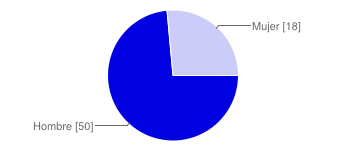
\includegraphics[width=10cm]{Resultados_Encuesta/Sexo.png} &
        \begin{tabular}{|c|cc|}
        \hline
         Hombre & 104 & 67\% \\ \hline
         Mujer & 51 &  33\%\\ \hline 
        \end{tabular} \\
      \end{tabular}
  \item Cual es su ocupación \\
      \begin{tabular}{m{10cm}m{5cm}}
        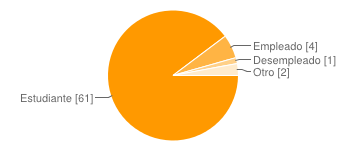
\includegraphics[width=10cm]{Resultados_Encuesta/Ocupacion.png} &
        \begin{tabular}{|c|cc|}
        \hline
         Estudiante & 102 & 66\% \\ \hline
         Empleado & 39 & 25\% \\ \hline 
         Desempleado & 3 & 2\% \\ \hline
         Otro & 11 & 7\% \\ \hline
        \end{tabular} \\
      \end{tabular}
  \item Cual de los siguientes elementos posee usted en la actualidad \\
      \begin{tabular}{m{7cm}m{5cm}}
        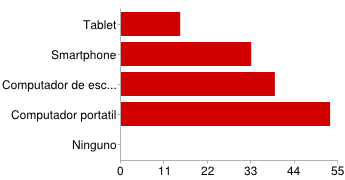
\includegraphics[width=7cm]{Resultados_Encuesta/Elementos.png} &
        \begin{tabular}{|c|cc|}
        \hline
         Tablet & 39 & 12\% \\ \hline
         Smartphone & 81 & 25\% \\ \hline
         Computador de escritorio & 85 & 26\% \\ \hline
         Computador portatil & 119 & 37\% \\ \hline
         Ninguno & 1 & 0\% \\ \hline
        \end{tabular} \\
      \end{tabular}
  \item ¿Desde qué lugar suele usted acceder a internet? \\
      \begin{tabular}{m{8cm}m{5cm}}
        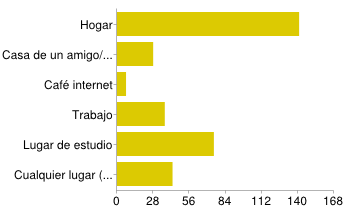
\includegraphics[width=8cm]{Resultados_Encuesta/Lugar.png} &
        \begin{tabular}{|c|cc|}
        \hline
         Hogar & 141 & 43\% \\ \hline
         Casa amigo & 28 & 8\% \\ \hline
         Café internet & 7 & 2\% \\ \hline
         Trabajo & 37 & 11\% \\ \hline
         Lugar de estudio & 75 & 23\% \\ \hline
         Cualquier lugar & 43 & 13\% \\ \hline
        \end{tabular} \\
      \end{tabular}
  \item ¿Cual es el lugar desde el cual usted dura mas tiempo navegando por internet? \\
      \begin{tabular}{m{8cm}m{5cm}}
        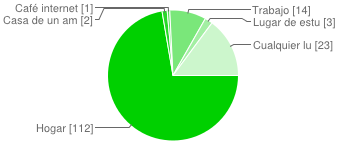
\includegraphics[width=8cm]{Resultados_Encuesta/Lugar_mayor.png} &
        \begin{tabular}{|c|cc|}
        \hline
         Hogar & 112 & 72\% \\ \hline
         Casa amigo & 2 & 1\% \\ \hline
         Café internet & 1 & 1\% \\ \hline
         Trabajo & 14 & 9\% \\ \hline
         Lugar de estudio & 3 & 2\% \\ \hline
         Cualquier lugar & 23 & 15\% \\ \hline
        \end{tabular} \\
      \end{tabular}
  \item En promedio, ¿Cuanto tiempo utiliza usted el internet por dia? \\
      \begin{tabular}{m{10cm}m{5cm}}
        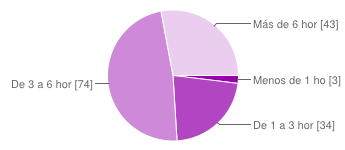
\includegraphics[width=10cm]{Resultados_Encuesta/Tiempo.png} &
        \begin{tabular}{|c|cc|}
        \hline
         Menos de 1 hora & 3 & 2\% \\ \hline
         De 1 a 3 horas & 34 & 22\% \\ \hline
         De 3 a 6 horas & 74 & 48\% \\ \hline
         Mas de 6 horas & 43 & 28\% \\ \hline
        \end{tabular} \\
      \end{tabular}
  \item ¿Practica usted algún deporte? \\
  \begin{tabular}{m{10cm}m{5cm}}
        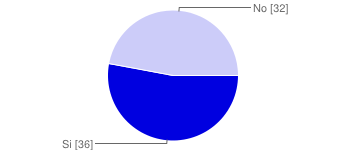
\includegraphics[width=10cm]{Resultados_Encuesta/Practica_deporte.png} &
        \begin{tabular}{|c|cc|}
        \hline
         Si & 98 & 63\% \\ \hline
         No & 57 & 37\% \\ \hline
        \end{tabular} \\
      \end{tabular}
  \item En caso de practicar algún deporte, ¿Qué deporte practica? \\
      \begin{tabular}{m{8cm}m{5cm}}
        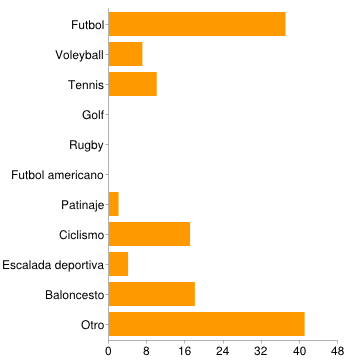
\includegraphics[width=8cm]{Resultados_Encuesta/Deporte.png} &
        \begin{tabular}{|c|cc|}
        \hline
         Fútbol & 37 & 27\% \\ \hline
         Voleyball & 7 & 5\% \\ \hline
         Tenis & 10 & 7\% \\ \hline
         Golf & 0 & 0\% \\ \hline
         Rugby & 0 & 0\% \\ \hline
         Fútbol americano & 0 & 0\% \\ \hline
         Patinaje & 2 & 1\% \\ \hline
         Ciclismo & 17 & 13\% \\ \hline
         Escalada deportiva & 4 & 3\% \\ \hline
         Baloncesto & 18 & 13\% \\ \hline
         Otro & 41 & 30\% \\ \hline
        \end{tabular} \\
      \end{tabular}
  \item Cuando quiere buscar personas con quien practicar deporte ¿Por qué medio lo hace? \\
      \begin{tabular}{m{8cm}m{5cm}}
        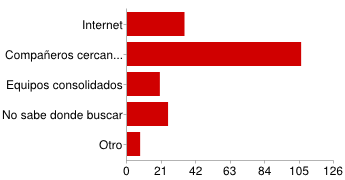
\includegraphics[width=8cm]{Resultados_Encuesta/Buscar_persona.png} &
        \begin{tabular}{|c|cc|}
        \hline
         Internet & 35 & 18\% \\ \hline
         Compañeros cercanos & 106 & 55\% \\ \hline
         Equipos consolidados & 20 & 10\% \\ \hline
         No sabe donde & 25 & 13\% \\ \hline
         Otro & 8 & 4\% \\ \hline
        \end{tabular} \\
      \end{tabular}
  \item Cuando quiere buscar un lugar donde practicar deporte ¿Por qué medio lo hace? \\
      \begin{tabular}{m{8cm}m{5cm}}
        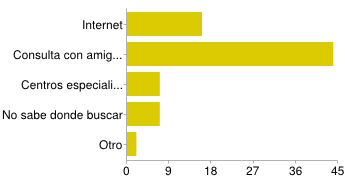
\includegraphics[width=7cm]{Resultados_Encuesta/Buscar_lugar.png} &
        \begin{tabular}{|c|cc|}
        \hline
         Internet & 48 & 24\% \\ \hline
         Amigos & 96 & 48\% \\ \hline
         Centros especializados & 32 & 16\% \\ \hline
         no sabe donde & 17 & 9\% \\ \hline
         Otro & 7 & 4\% \\ \hline
        \end{tabular} \\
      \end{tabular}
  \item Cuando quiere buscar implementos deportivos, ¿Por qué medio lo hace? \\
      \begin{tabular}{m{8cm}m{5cm}}
        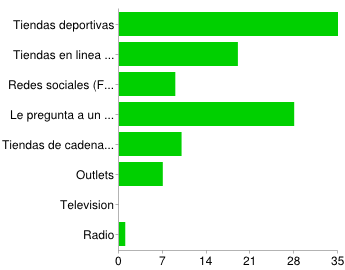
\includegraphics[width=8cm]{Resultados_Encuesta/Buscar_implemento.png} &
        \begin{tabular}{|c|cc|}
        \hline
         Tiendas deportivas & 89 & 32\% \\ \hline
         Tiendas en linea & 54 & 19\% \\ \hline
         Redes sociales & 27 & 10\% \\ \hline
         Pregunta a conocido & 59 & 21\% \\ \hline
         Tiendas de cadena & 30 & 11\% \\ \hline
         Outlets & 19 & 7\% \\ \hline
         Televisión & 1 & 0\% \\ \hline
         Radio & 1 & 0\% \\ \hline
        \end{tabular} \\
      \end{tabular}
      \newpage
  \item Cuando quiere buscar un nuevo deporte para practicar, ¿Por qué medio lo hace? \\
      \begin{tabular}{m{8cm}m{5cm}}
        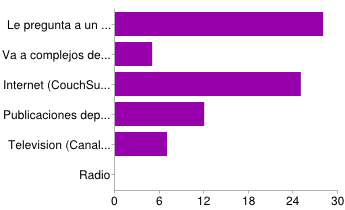
\includegraphics[width=8cm]{Resultados_Encuesta/Buscar_deporte.png} &
        \begin{tabular}{|c|cc|}
        \hline
         Pregunta a conocido & 57 & 33\% \\ \hline
         Va a complejos deportivos & 21 & 12\% \\ \hline
         Internet & 60 & 34\% \\ \hline
         Publicaciones deportivas & 24 & 14\% \\ \hline
         Televisión & 13 & 7\% \\ \hline
         Radio & 0 & 0\% \\ \hline
        \end{tabular} \\
      \end{tabular}
  \item Usted quiere practicar un deporte nuevo, ¿Cómo prefiere hacerlo? \\
      \begin{tabular}{m{10cm}m{5cm}}
        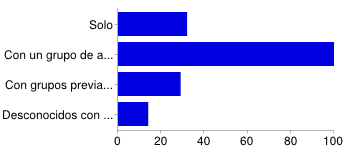
\includegraphics[width=10cm]{Resultados_Encuesta/Nuevo_deporte.png} &
        \begin{tabular}{|c|cc|}
        \hline
         Solo & 32 & 18\% \\ \hline
         Grupo de amigos & 100 & 57\% \\ \hline
         Grupos consolidados & 29 & 17\% \\ \hline
         Desconocidos & 14 & 8\% \\ \hline
        \end{tabular} \\
      \end{tabular}
  \item BONUS: ¿Considera usted que los videojuegos sean un deporte? \\
      \begin{tabular}{m{10cm}m{5cm}}
        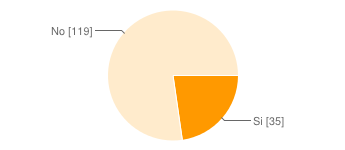
\includegraphics[width=10cm]{Resultados_Encuesta/Bonus.png} &
        \begin{tabular}{|c|cc|}
        \hline
         Si & 35 & 23\% \\ \hline
         No & 119 & 77\% \\ \hline
        \end{tabular} \\
      \end{tabular}
\end{itemize}

  
  
  
\end{document}
